%---------------------------------------------------------------------
% Please do not modify anything in this box!                         |
% -------
\documentclass[a4paper, 11pt]{article}
\usepackage{radioprop}
\usepackage{graphicx}
\usepackage{xcolor}
\usepackage[square, numbers]{natbib}

\newcommand{\cw}[1]{\textbf{\color{red} CW: #1}}
\newcommand{\FC}[1]{\textbf{\color{purple} FC: #1}}

%-------------------------------------------------------------------
\begin{document}
%-------------------------------------------------------------------
%
\parabole
%
%
%-------------------------------------------------------------------
% Title (insert one line only)
%-------------------------------------------------------------------
\title{Searches for Axion Dark Matter with the Sardinia Radio Telescope}
%------- ---------------------------------------------------------
% Principal Investigator (including name, address, telephone, fax, email)
%----------------------------------------------------------------
\pifirstname{Andrea}
\pilastname{Possenti}
\piinstitute{INAF-Osservatorio Astronomico di Cagliari}
\pistreetandnumber{via della Scienza 5}
\pizipandcity{09047 - Selargius}
\picountry{Italy}
\piphone{+39 070 71180228}
\pifax{+39 070 71180222}
\piemail{andrea.possenti@inaf.it}
%----------------------------------------------------------------
% Coauthors 
% macro: \coauthor{First_Name Last_Name}{affiliation} 
% use one \coauthor{ }{ } macro for each coauthor. 
% You may add as many \coauthor{ }{ } macros as needed ...
%----------------------------------------------------------------
\coauthor{Christoph Weniger}{University of Amsterdam}
\coauthor{Ben Safdi}{University of Michigan}
\coauthor{Francesca Calore}{CNRS, LAPTh}
\coauthor{Gregory Desvignes}{MPIFR, Bonn}
\coauthor{Ralph Eatough}{MPIFR, Bonn}
\coauthor{Yonatan Kahn}{University of Chicago}
\coauthor{Vlad Kondratiev}{ASTRON-Dwingeloo}
\coauthor{Alessandro Corongiu}{INAF-OACagliari}
\coauthor{Silvia Leurini}{INAF-OACagliari}
\coauthor{Delphine Perrodin}{INAF-OACagliari}
\coauthor{Fabrizio Tamburini}{}
% ...
%----------------------------------------------------------------
%
\observer{Corongiu, Leurini, Perrodin, Possenti}                    
%-------------------------------------------------------------------
% Choose one of the following keywords which describes project contents best
\astronomy
%\geodesy
%\spacescience
%\telescopetest
%
%\resubmit{}       % Is this a resubmission of a previous proposal? (Ref.number)
%\continue{}       % Is this a continuation of a previous proposal? (Ref.number)
%\studentname{}   % Is this for a Ph.D. project? (Student's name)t
%-------------------------------------------------------------------
% Amount of time 
%-------------------------------------------------------------------
% this  proposal
\hours{3}                        
% {for full completion} {already allocated}
\totalhours{3}{0}
%-------------------------------------------------------------------
% Sidereal time intervals:  {start} {end} {number of intervals}
%-------------------------------------------------------------------
\lsta{15:00}{21:00}{2}
%\lstb{}{}{}
%-------------------------------------------------------------------%---------------------------------------------------------------------
\sciabstract{Astrophysical observations of galaxies and galaxy clusters, and cosmological observations of the temperature fluctuations of the cosmic microwave background provide strong evidence for the existence of dark matter (DM) in the Universe.  One of the oldest and theoretically best motivated DM candidates are QCD \textit{axions}, ultralight particle that solve the strong CP problem of the Standard Model of particle physics.  For masses in the $\mu$eV range, these particles also naturally explain the observed amount of cold DM. Substantial experimental efforts are underway to search for these particles in laboratory experiments.  Here, we propose to leverage on the fact that DM axions can resonantly convert into photons when traversing the strong magnetic field in the magnetosphere of neutron stars (NS).  The observable signal is a narrow spectral line, with frequency that depends on the (unknown) axion mass.  Detailed calculations show that slowly-spinning NSs lead to the most efficient conversion.  An optimal target for axion searches is hence the large population of dead NSs, which can be inferred from population synthesis arguments.  We propose here to use the Sardinia Radio Telescope to search for narrow spectral lines from the Galactic center (GC) region, using P- and L-band receivers.  The proposed searches would be complementary to similar work with the Effelsberg telescope.  A discovery of an axion line would be a major breakthrough, but even null results would provide the (by far) strongest limits on the axion photon coupling and will significantly deepen our understanding of DM in the Universe.
}


%-------------------------------------------------------------------
\outabstract{Dark matter is a mysterious substance that is thought to account for about 85\% of all mass in the Universe.  Its gravitational effects can be clearly seen in galaxies and galaxy clusters today.  To our best understanding, dark matter played a central role in the formation of these objects, supporting their growth from the tiny density variations of the primordial plasma that we can still infer from the cosmic microwave background.  One of the most plausible candidates for DM are ultralight particles, so-called axions, which were proposed to cure some shortcomings of the Standard Model of particle physics. Such particles are linked to the electromagnetic force in subtle ways, which allow the conversion of DM axions into photons in the presence of strong magnetic fields.  We search for such conversion in the enormously strong magnetic fields that accompany neutron stars. This approach will allow us to probe previously unexplored mass ranges of the DM axion hypothesis, bringing us one step (and in the case of a discovery, a giant leap) further in the long quest for particle DM.
}
%----------------------------------------------------------------
% The following command will actually produce the front page. 
%----------------------------------------------------------------
\frontpage
%
%----------------------------------------------------------------
% Scientific justification 
% (max. 2 pages of text plus 2 pages of Figs., Tables and Refs.)
%----------------------------------------------------------------
% Please consider the following scheme

\section*{Scientific Background and State of the Art}
%  Describe the general scientific context of your project, elaborate the 
%  present problems in the field and motivate your solution to these problems

The gravitational evidence for dark matter (DM) in the Universe is overwhelming, but there is as of yet no unambiguous evidence of non-gravitational interactions of DM with ordinary matter.   One of the most promising DM candidates is an ultralight particle called the axion (Irastorza et al 2018, Beringer et al ????).   A priori, the axion mass $m_a$ is a free parameter of the model.  However, the mass range which naturally explains the observed DM abundance is roughly between $m_a = 10^{-7}$ eV and $m_a = 10^{-4}$ eV.   Laboratory searches for axion DM with resonant cavity experiments like ADMX probe already parts of this range.  These searches will be further extended over the coming years~(Du et al. 2018, Ph. Rev. L. 120, 151301).  

The axion couples extremely weakly to ordinary matter, via  subtle modifications to Maxwell's equations (see e.g. Graham 2015 for a review).  In particular, DM axions can convert into electromagnetic waves in the presence of static, external magnetic fields.  The frequency of the electromagnetic radiation is given by $f = m_a c^2 (1 + v^2 / 2 c^2) / (2 \pi \hbar)$, where $c$ is the speed of light, $\hbar$ is the reduced Planck constant, and $v$ is the relative velocity of the astrophysical DM ($v \sim 200$ km$/$s locally).  This means that axions in the mass range quoted above could in principle give rise to radio lines in the frequency range 20 MHz -- 20 GHz, accessible by current radio telescope technology.

DM axions may convert into electromagnetic radiation in the strong magnetic fields permeating NS magnetospheres~(e.g. Pshirkov et al. 2007, Hook et al. 2018).  The predicted signal is a narrow line (typically $B / f \sim 10^{-6}$ for individual NSs, where $B$ is the line bandwidth and $f$ the central frequency of the line), and all NSs should radiate at the same (but currently unknown) frequency, set by the axion mass.   Here, we will focus on the inner region of the Galaxy, where we can benefit from observing the summed contribution from emission of all NSs expected within the field of view.  Since the NSs themselves all emit at the same frequency, which is however Doppler shifted by the velocity dispersion of the source population, the relative bandwidth of the combined signal increases significantly to $B /f \sim 10^{-3}$~(Chen, Safdi, Sun in press), corresponding to line width of $\sim 0.3-1$ MHz for lines in the P and L bands. It was shown in Hook et al. (2018) that radio telescopes may indeed achieve competitive sensitivity to terrestrial experiments searching for axion DM.


\section*{Goals of the Proposed Observations}

In this proposal, we will leverage on the fact that neutron stars (NSs) should produce radio lines in the presence of axion DM~(Pshirkov et al. 2007, Hook at al. 2018), covering regions of the axion DM parameter space that are complementary to the ADMX effort and other searches.   \textbf{We propose to use the SRT to search for narrow radio lines resulting from axion DM conversion in NS magnetospheres in the frequency ranges 300 - 360 MHz and 1.3 -- 1.8 GHz \FC{in the direction of the GC}}, see Tab.~\ref{tab:label}.  In total, we are requesting 2 hours of on-target observation time.  Each on-target observation will be 30 minutes long.   \textbf{This work has the potential to provide the first evidence for particle DM.  However, even a null result will lead to new and world-leading constraints on axion DM.} 

\medskip
 
In Fig.~1, we show the sensitivity that will be achieved by the searches in this proposal to current and projected constraints on axion DM. Our sensitivities are derived by requiring a signal-to-noise ratio of 10, using the radiometer equation, with the sky temperature derived from the Haslam 408 MHz map, using a spectral index of $-2.6$.  The signal fluxes are calculated using the formalism from Hook at al. (2018) and Chen, Safdi \& Sun (in press).  We are here interested in the combined emission of old slow neutron stars in the inner galaxy; their number density, period and magnetic field distributions can be estimated from the star formation history in the Galactic bulge and nuclear star cluster, combined with models for pulsar evolution that have been tuned to the available X-ray and radio data~(Chen, Safdi \& Sun, in press).  One of the largest sources of uncertainty in the calculation of the GC flux is the DM profile in the inner regions of the Milky Way, though uncertainties on the NS population model are also important.   Since the emission from the GC, and slightly offset from the GC, are affected by different systematics and different foregrounds, we propose to observe two different target regions (GC and `GC offset', $1^\circ$ north of the GC) with the same exposure.

The $y$-axis shows the unknown coupling strength $g_{a \gamma \gamma}$ between the axion and electromagnetism.  The conversion probability between axions and photons is proportional to $g_{a \gamma \gamma}^2$.  The best-motivated region of parameter space is shown in orange.  There, the axion simultaneously explains the absence of the neutron electric dipole moment (in this region the axion is called the ``QCD axion'') and the cold dark matter abundance.  However, axion(-like particles) DM may in fact inhabit any part of the parameter space, as occurs for example in models inspired by string theory~\cite{Svrcek:2006yi}.    

The upper grey-green band in Fig.~\ref{fig: sensitivity} was excluded by the CAST experiment~\cite{Arik:2015cjv}, which searches for axions produced in the Sun.  The only part of the QCD axion parameter space excluded so far is the dark red region, representing constraints from the ADMX experiment~\cite{Du:2018uak}.  The long-term plan of the ADMX program is to cover the lightly-shaded red region, though we emphasize that that parameter space is still allowed today.  As clearly seen in Fig.~\ref{fig: sensitivity}, the searches detailed in this proposal will cover a significant region of currently unprobed axion DM parameter space, while setting the stage for future observations that could eventually probe the QCD axion couplings. 

The modest observation time of 30 minutes per source is already sufficient to set world-leading limits on axion DM in this frequency range (see Fig.~\ref{fig: sensitivity}). We note that a positive result would be spectacular and strong evidence for the existence of axion DM.  However, in this field, null results are also of the utmost importance because they determine where future experiments and observations should focus their efforts. 

%We will use an integration time of 100 ms \cw{Possible?} corresponding to a data-taking rate of XXX MB/s per spectrometer.  Such high time resolution is necessary because the signal from the magnetar is expected to be pulsed at the NS rotational rate, with periods of the order $\sim$10 s.

%In addition, we will also search for the much more narrow line $B/f\sim 10^{-6}$ associated with the Galactic center magnetar PSR J1745-2900.

\medskip

We stress that observations especially with the SRT would be highly valuable, since the possible frequency coverage is \textit{complementary} to the frequencies covered by similar ongoing searches using the Effelsberg radio telescope.  At the same time, SRT still provides a comparable forward gain.  These two facts allow to significantly increase the axion model parameter space probed by radio searches, even with the relatively little requested observation time.  More specifically, for our purposes Effelsberg data is only available above 2 GHz (since they are connected to the regular magnetar observations of the GC which are only performed at high frequencies).  The proposed P- and L-band with SRT observations would help to cover lower frequencies.  %Furthermore, the frequency range 5.7 -- 7.7 GHz of the SRT C-high receiver is not covered by any of the working receiver configurations at Effelsberg.  Again, such observations would help to will the gaps.  
Finally, preliminary high-resolution S-band data that we have available from Effelsberg allowed us to explore how well axion DM signals could in principle be discriminated from actually radio frequency interference (RFI).  This experience inspired the configuration proposed in Tab.~\ref{tab:label} (more details below).


\section*{Feasibility and Time Estimate}
%  Demonstrate that these observations will be feasible with the selected 
%  technical setup and provide all technical details required to reproduce
%  your time request.

%In order to detect the narrow-band signal from the magnetar, while still covering a wide range of frequencies, 

Part of the frequency range of interest is known to be heavily affected by RFI.   For the corresponding frequencies the sensitivity to axion DM signals would be reduced.  
%Sightlines through the Galaxy in this band are likely to include velocity shifted HI and OH maser lines; these will have comparable widths to the expected signals in the population targets, but vary from sightline to sightline.  
%Rather than attempting to change the observational setup for each target to avoid them, we will exclude affected frequencies from the searched spectra during the data processing.  
%
Using preliminary S-band data from the Effelsberg telescope (2 kHz channel width), we found that although parts of the frequency range were strongly affected by RFI, none of the strong RFI lines was compatible with the specific Doppler broadened spectral line expected from the combined emission of NSs in the Galactic center region.  Weaker line candidates in the data could be still rejected due to their presence in the off region observations.  We found that even when the observed uncertainties are folded back into the upper limit calculations, these upper limits where over the majority of the explored frequency range comparable to the expected constraints derived by the radiometer equation.

From the above experience, we conclude that in order to optimize the handling of RFI, we need a high spectral resolution and position switching.  Naively, this would suggest using baseband observations with ROACH1.  However, the limited BW of ROACH1 (128 MHz) allows this only for the P-band receiver.  For L-band we hence plan to use the SARDARA back-end, with the maximum number of channels and BW, as shown in Tab.~\ref{tab:label}.  This would still allow us to resolve signal candidate lines.  Since the NS signal of interest is not expected to be significantly pulsed (at least for our purposes), we will use integration times of 1 minute to further increase the handling of time-varying RFI. For the position switching, we propose a single off target position $10^\circ$ north of the GC, which will avoid any contribution from possible signal emission.  This region will serve as off region both for the GC and the `GC offset' observations.

\paragraph{Management and Resources.} The overall project will be under the direction of the PI A.~Possenti, who has experience with collecting and analyzing data from the SRT, and by co-PI C.~Weniger, with experience in laboratory and astrophysical searches for DM.
A. Corongiu, S. Leurini and D. Perrodin will help with observations and initial data reduction. G.~Desvignes, R.~Eatough and V.~Kondratiev, who are all experienced radio astronomers, will also help analyzing the data; B.R.~Safdi, F.~Calore and Y.~Kahn, who are experts on DM, will focus on the DM interpretation.  


\paragraph{Technical justification.}

The signal flux corresponding to a signal-noise-ratio of 10 is calculated as follows:  $S_{\rm sig} = 10\cdot T_{\rm sys}/G/\sqrt{T_{\rm obs} B}$, where $T_{\rm sys} = T_{\rm rx} + T_{\rm sky}$, $T_{\rm rx} = 30(65) \rm\; K$ for L-band (P-band), $T_{\rm sky} = 200(600) \rm\; K$ for GC and $T_{\rm sky} = 50(150) \rm\; K$ for `GC offset' observations, $G = 0.55(0.52) \rm\; K/Jy$, $B \simeq 10^{-3} f$, $f$ is the line frequency, and $T_{\rm obs} = 1800 \rm\; s$ the observation time.  For the Galactic center observations at L-band, we find for example $S_{\rm sig} = 0.23\rm\; Jy$.  The results where double-checked using the online sensitivity calculator for the SRT (only available for L-band).  We note that observation will happen with a channel size that is significantly smaller than the signal bandwidth $B$.  The above estimate takes into account that during the actual line analysis channels will be either optimally re-binned, and/or a maximum-likelihood analysis will be performed    .


\section*{Re-allocation to a Different Antenna}
%  Declare whether your program is suitable for possible re-allocation to one of
%  the other antennas, in case the preferred one is unavailable - e.g. because
%  higher-rank programs are filling the schedule or unexpected technical issues 
%  arise. If choosing this option, specify in this section the increase (or reduction)
%  in observing time - for each target - that is needed to obtain the original scientific goals. 

In order to achieve the scientific goals of this project, observations with SRT are essential.  The receivers available at the Medicina or Noto telescopes do not cover the frequency ranges of interest (in particular not P-band), and they do not have the required large number of channels for RFI-signal separation.  Finally, the much lower forward gain of the instrument would make it necessary to increase the observation time by a factor 20 and more to achieve the same sensitivity goals.  

\clearpage

\bibliographystyle{JHEP}
\bibliography{axion}

\begin{figure}
   \centering
  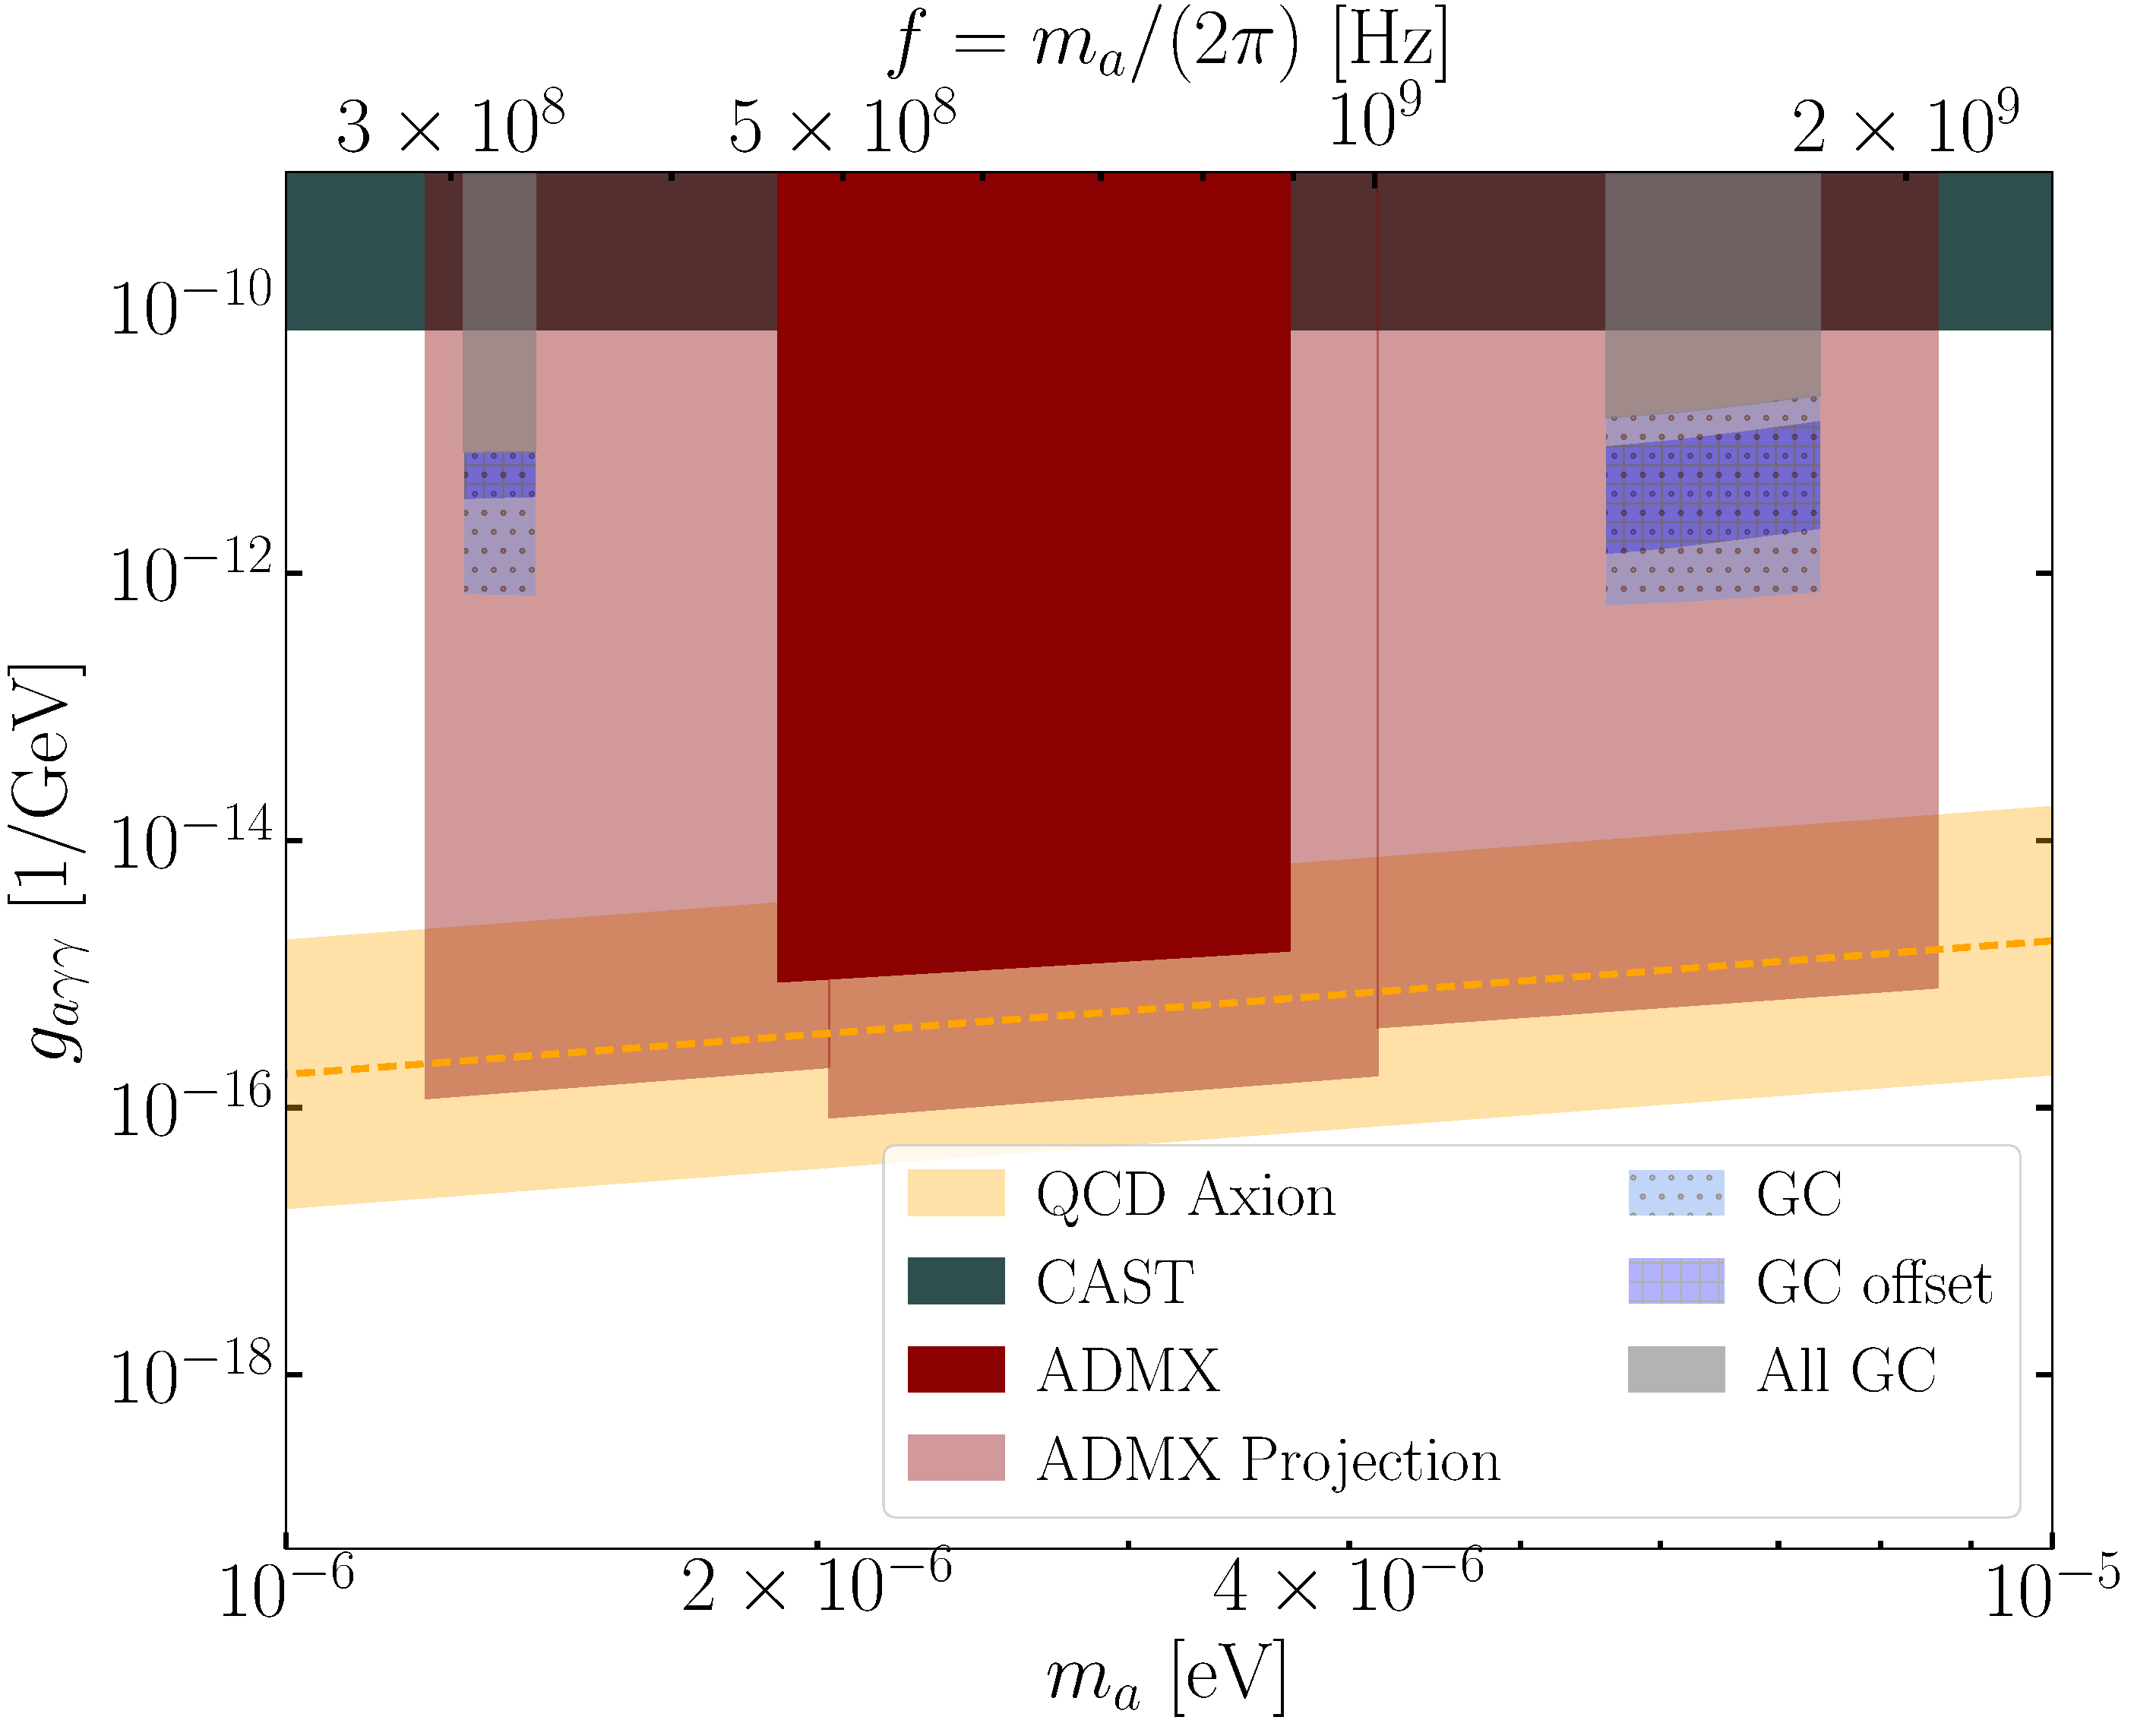
\includegraphics[width=0.50\textwidth]{SRT_GC.pdf}
   \caption{Sensitivity to axion-photon coupling for signal-to-noise ratio of 10 using the SRT P- and L-band receivers (Tab.~\ref{tab:label}), alongside existing constraints and favored regions.  The signal flux is estimated based on population synthesis arguments for old NSs in the inner Galaxy, both for GC observations and observations of the GC with a $1^\circ$ offset (where the dark matter density is less uncertain and the sky temperature significantly lower).  The bands show uncertainties in the expected sensitivity reach due to uncertainties in the dark matter density in the inner galaxy.  The dark red and gray regions are already excluded, the light red region shows the expected reach of laboratory searches during the next 10 years.  Searches with radio telescopes allow to probe part of this parameter space already now.  The yellow band shows couplings expected for the most popular QCD axion models, however in general axion DM is possible over the entire shown parameter space.  See text for details.
}
   \label{fig: sensitivity}
   \end{figure}
   
\begin{table*}[htb]
  \centering
  \caption{List of targets proposed for observations.  Indicated observation times correspond to on-target times. Position switching will increase these times by a factor of 1.5, leading to a total of 3 requested hours of telescope time.  `GC' corresponds to the Galactic center (Sgr A$^\ast$), `GC offset' is $1^\circ$ north of the Galactic center.  Signal predictions are affected by different systematics (mostly related to the DM density), and the combined observation of two regions (GC and GC offset) helps to make the results more robust.  
  \label{tab:label}
  }
  \vskip 2mm
  \begin{tabular}{lrrrrrr}
    \hline
    Target & $T_{\rm obs}$ [min] & Frequencies & Receiver & Back-end & Usable Bandwidth & $N_{\rm channel}$ \\
    \hline
    \hline
    GC & 30 & 300 -- 360 MHz & P & ROACH1 & 64 MHz & $10^5$  \\
    GC & 30 & 1.3 -- 1.8 GHz & L & SARDARA & 400 MHz & 16384  \\
    GC offset & 30 & 300 -- 360 MHz & P & ROACH1 & 64 MHz & $10^5$ \\
    GC offset & 30 & 1.3 -- 1.8 GHz & L & SARDARA & 400 MHz & 16384  \\
    %GC & 30 & 5.7 -- 6.7 GHz & C-high & SARDARA & 1500 MHz & 16384 & \\
    %GC & 30 & 6.7 -- 7.7 GHz & C-high & SARDARA & 1500 MHz & 16384 & \\
    %GC & 17:45 & $-$29 & 15 & 0.3 -- 0.5 / 0.5 -- 1.0 & P500\\
    %GC & 17:45 & $-$29 & 15 & 0.8 -- 1.3 (RFI!) & P300\\
   %GC & 17:45 & $-$29 & 15 & 1.27 -- 1.45 & P217\\
   %GC & 17:45 & $-$29 & 15 & 1.29 -- 1.43  / 1.57 -- 1.72 & P200\\
    %GC & 17:45 & $-$29 & 15 & 2.3 -- 2.8 & S110\\
    %GC & 17:45 & $-$29 & 15 & 4.5 -- 5.0 & S45\\
    %GC & 17:45 & $-$29 & 15 & 8.1 -- 8.6 & S36\\
    %GC & 17:45 & $-$29 & 15 & 10.3 -- 10.6 & S28\\
    \hline
  \end{tabular}
\end{table*}

\end{document}
